\documentclass{beamer}
\usetheme{metropolis}           % Use metropolis theme

\usepackage{braket}
\usepackage{amsmath}
\usepackage{cancel}
\usepackage{color}

\title{
  Precision nuclear structure in \\
  the in-medium similarity renormalization group
}
\date{\today}
\author{Matthias Heinz}
\institute{Institut f\"ur Kernphysik, TU Darmstadt}
\begin{document}

% TODO
\newcommand{\XXX}[1]{\textcolor{red}{#1}}

% Text shortcuts
\newcommand{\mscheme}{\texorpdfstring{$m$-scheme}{m-scheme}\xspace}
\newcommand{\abinitio}{\textit{ab initio}\xspace}

% Units
\newcommand{\mev}{\, \text{MeV}}
\newcommand{\invfm}{\, \text{fm}^{-1}}

% Second quant
\newcommand{\crea}[1]{\ensuremath{a_{#1}^{\dagger}}}
\newcommand{\annih}[1]{\ensuremath{a_{#1}}}
\newcommand{\qpcrea}[1]{\ensuremath{b_{#1}^{\dagger}}}
\newcommand{\qpannih}[1]{\ensuremath{b_{#1}}}

% Commutators
\newcommand{\comm}[2]{\ensuremath{[#1, #2]}}
\newcommand{\anticomm}[2]{\ensuremath{\{#1, #2\}}}

% A-body operators
\newcommand*{\zerobodyop}[1]{\ensuremath{{#1}^{(0)}}}
\newcommand*{\onebodyop}[1]{\ensuremath{{#1}^{(1)}}}
\newcommand*{\twobodyop}[1]{\ensuremath{{#1}^{(2)}}}
\newcommand*{\threebodyop}[1]{\ensuremath{{#1}^{(3)}}}
\newcommand*{\abodyop}[1]{\ensuremath{{#1}^{(A)}}}

% Normal ordering
\newcommand{\nogen}[1]{\ensuremath{\text{N}\left[#1\right]}}
\newcommand{\novac}[1]{\ensuremath{\text{N}_{0}\left[#1\right]}}
\newcommand{\noref}[1]{\ensuremath{\text{N}_{\Phi}\left[#1\right]}}

% Normal ordered operators
\newcommand*{\hnozero}{\zerobodyop{\bar{H}}}
\newcommand*{\hnoone}{\onebodyop{\bar{H}}}
\newcommand*{\hnotwo}{\twobodyop{\bar{H}}}
\newcommand*{\hnothree}{\threebodyop{\bar{H}}}


% Ref state
\newcommand{\refgnd}{\ensuremath{\ket{\Phi}}}
\newcommand{\refhp}[2]{\ensuremath{\ket{\Phi_{#1}^{#2}}}}

% IM_SRG generators
\newcommand*{\genone}{\eta^{(1)}}
\newcommand*{\gentwo}{\eta^{(2)}}
\newcommand*{\genthree}{\eta^{(3)}}

% m-scheme basis
\newcommand*{\emax}{e_{\text{max}}}

  \maketitle

  % \section{Motivation}

  \begin{frame}{\textit{Ab initio} nuclear structure}
    \begin{itemize}
      \item{Nuclei as made up of $A$ interacting nucleons}
      \item{Input (chiral) NN and 3N interactions \\ into (in limit) exact many-body method}
      \item{Advantages:}
      \begin{itemize}
        \item{General approach with large range of applicability}
        \item{Systematically improvable}
        \item{Rigorous estimation of uncertainties is possible}
      \end{itemize}
    \end{itemize}
  \end{frame}

  \begin{frame}{\textit{Ab initio} explosion}
    \begin{center}
      \begin{overprint}
        \onslide<1>\centering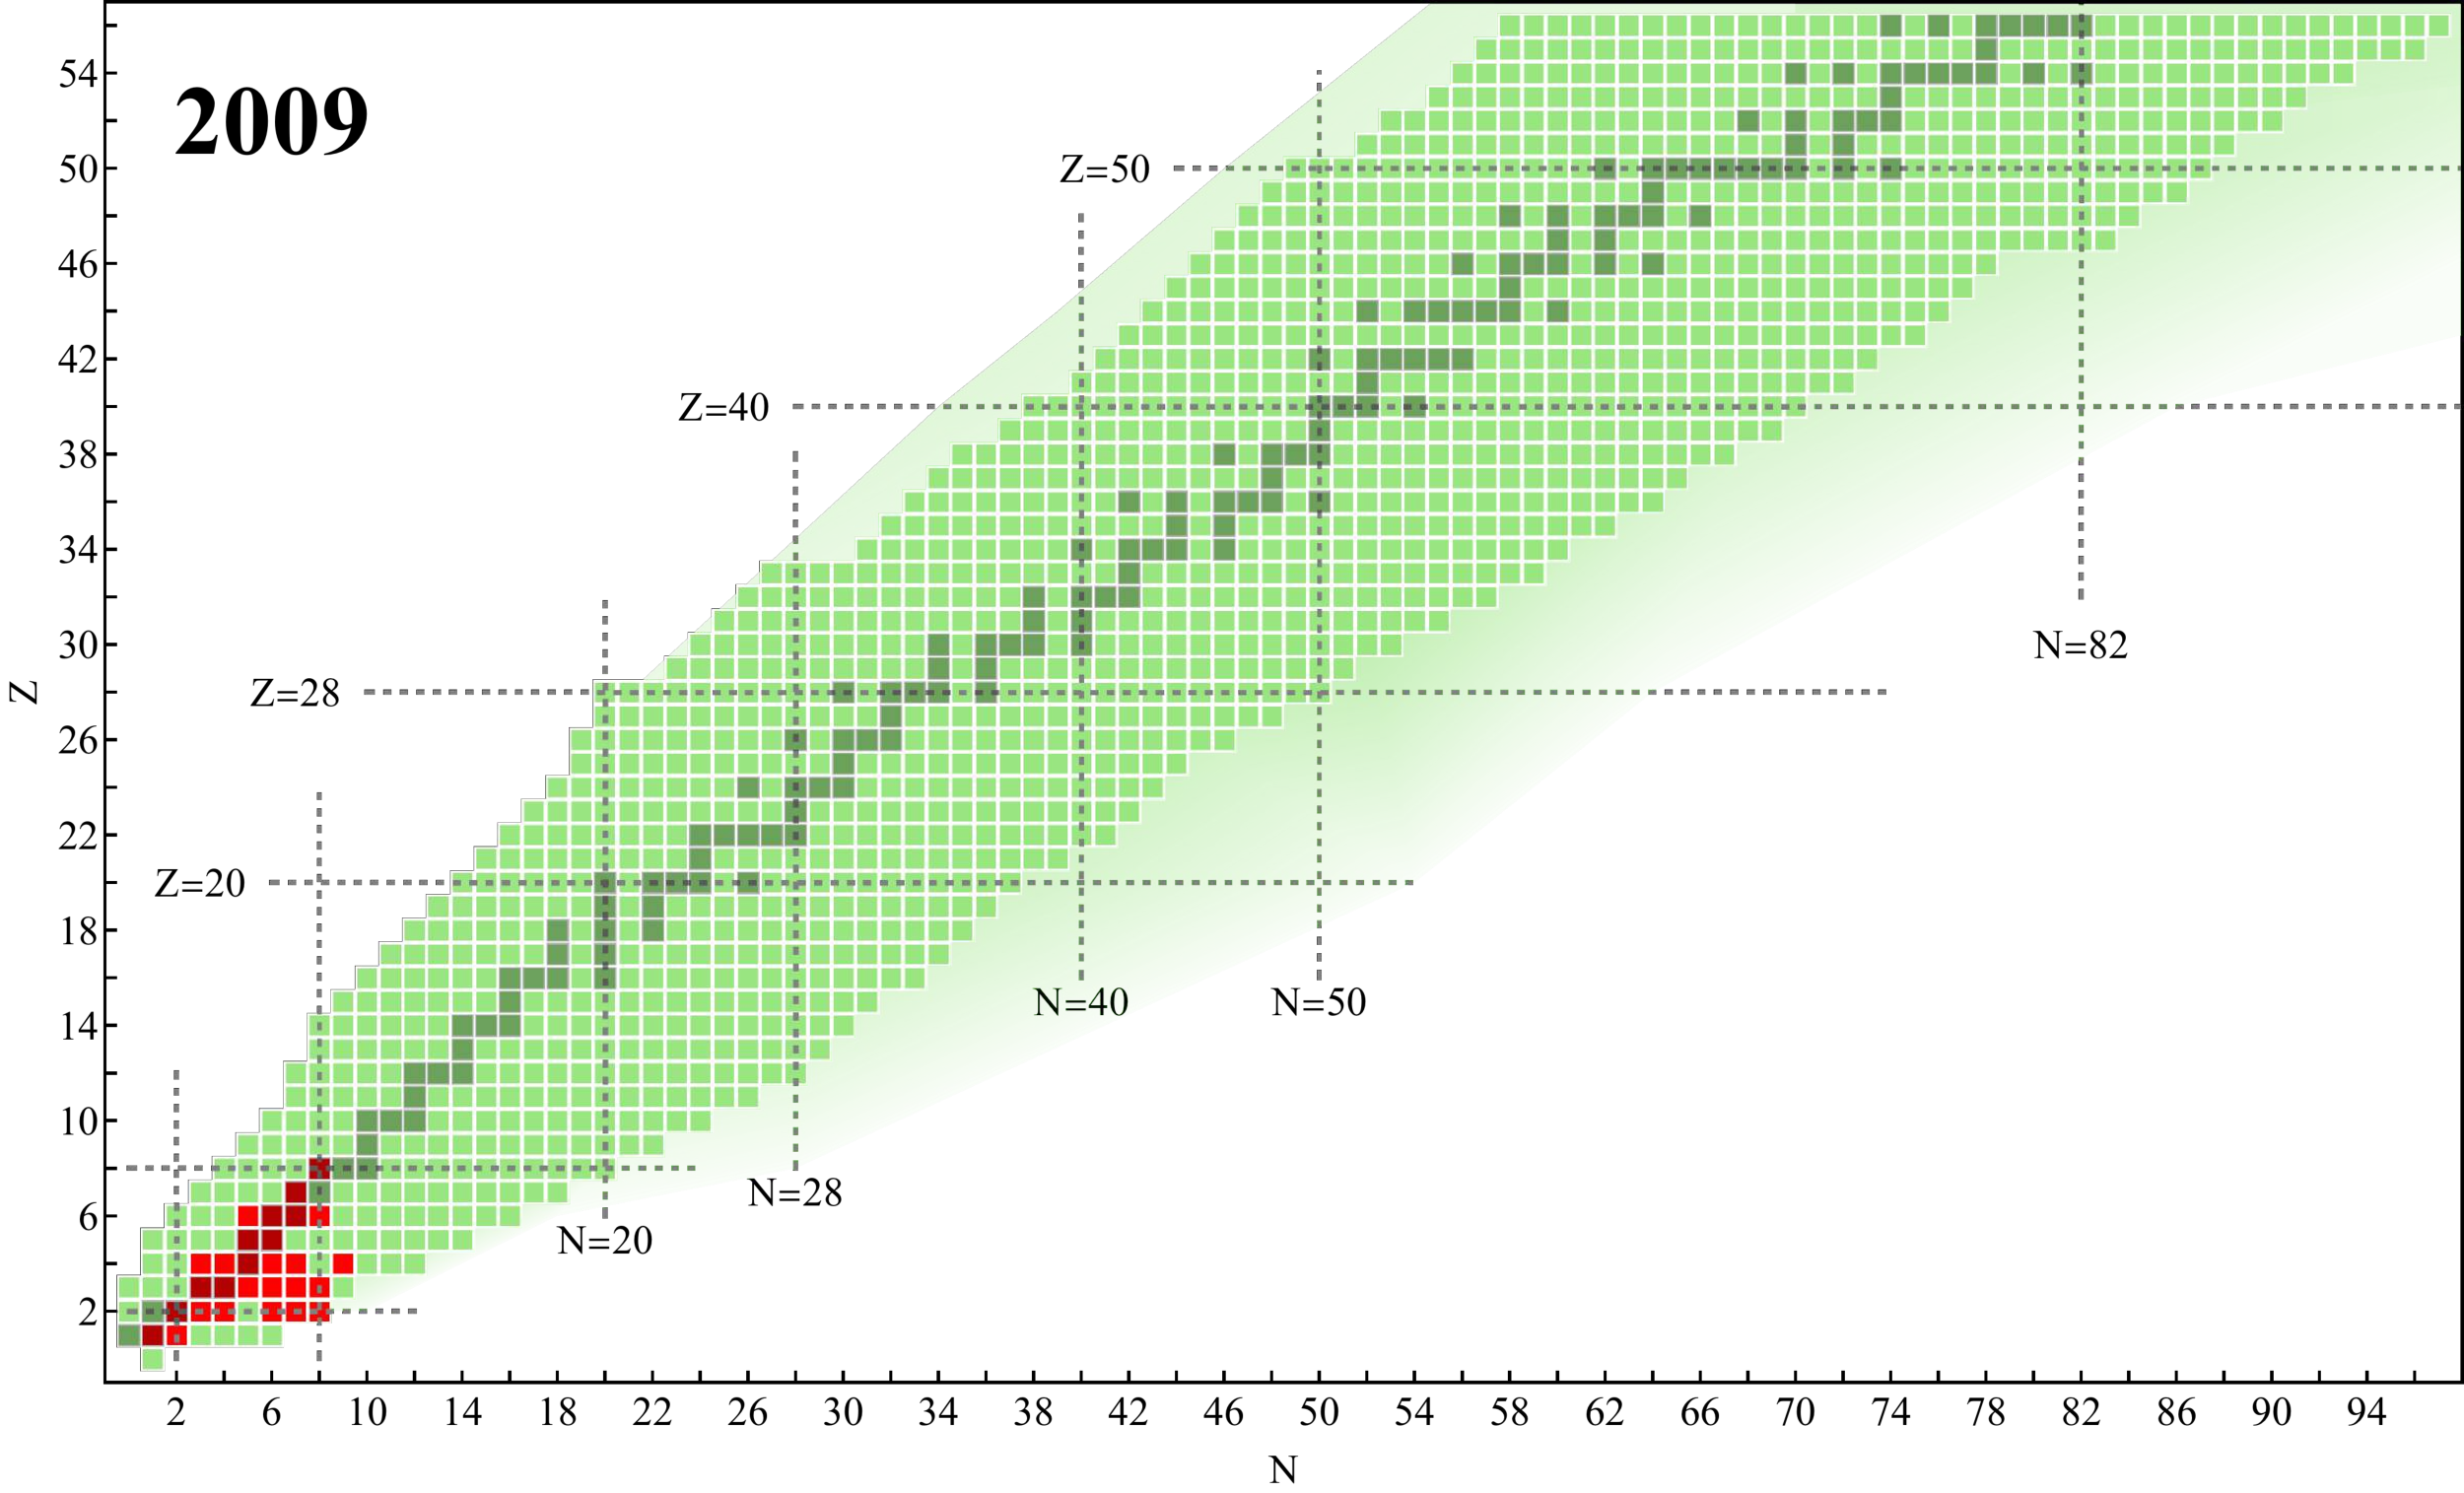
\includegraphics[width=0.8\textwidth]{proposal/talk/images/external/nuclear_chart_2009.pdf}
        \onslide<2>\centering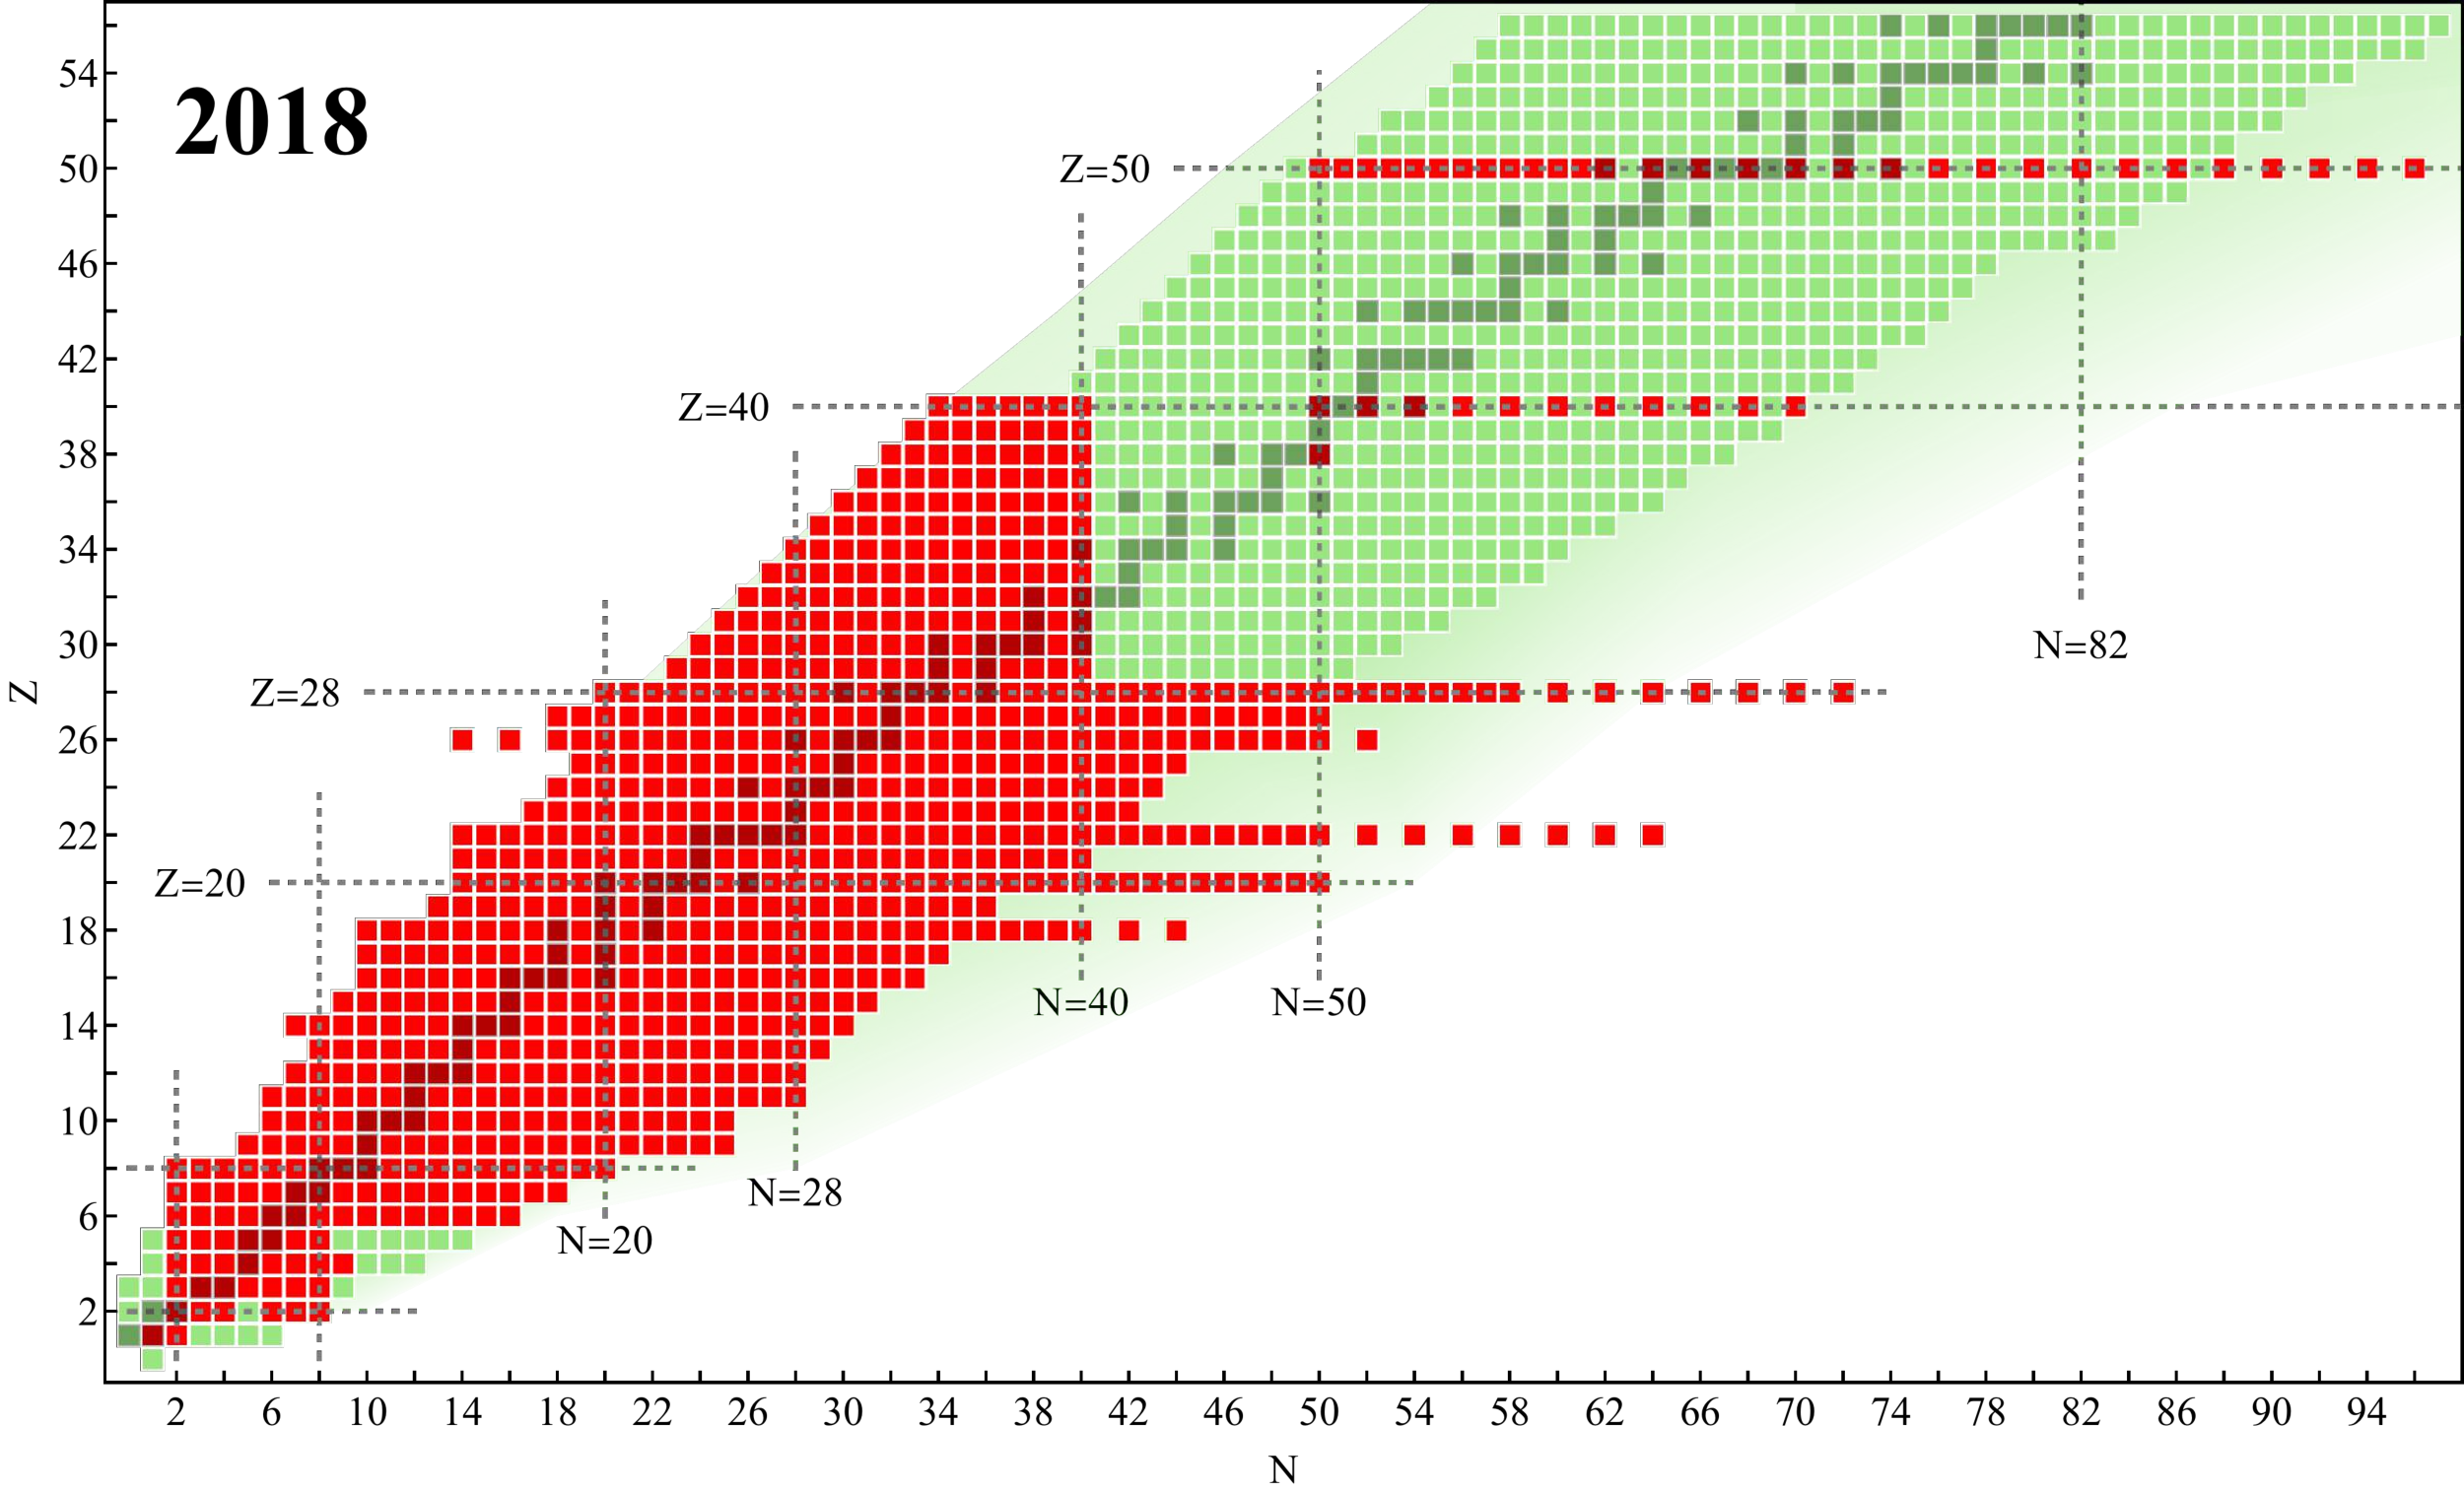
\includegraphics[width=0.8\textwidth]{proposal/talk/images/external/nuclear_chart_2018.pdf}
      \end{overprint}
      {\tiny Hebeler 2020, figure by Hergert}
    \end{center}
    \begin{itemize}
      \item{Low resolution interactions for low-energy physics}
      \item{Developments in many-body methods}
    \end{itemize}
  \end{frame}

  \begin{frame}{Current state of \textit{ab initio} theory}
    \begin{itemize}
      \item{Exact diagonalization (NCSM)}
      \begin{itemize}
        \item{Factorial scaling}
        \item{Only modelspace truncation}
      \end{itemize}
      \item{Many-body expansion methods}
      \begin{itemize}
        \item{MBPT, CC, IM-SRG, SCGF}
        \item{Single-particle basis truncation \\
          and truncation in many-body method}
        \item{Going to higher orders in many-body method \\
          is a substantial amount of work}
        \item{IM-SRG current status: IM-SRG(2)}
      \end{itemize}
    \end{itemize}
    \vskip1em
    Target: \textbf{IM-SRG(3)}
  \end{frame}

  % \section{Formalism}

  \begin{frame}{Similarity renormalization group}
    \begin{center}
      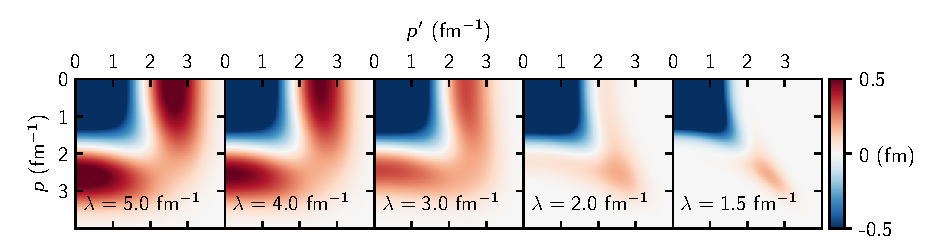
\includegraphics[width=\textwidth]{proposal/talk/images/vnn_srg_emn500_n3lo.pdf}
    \end{center}
    Continuous unitary transformation:
    \begin{equation*}
      H(s) = U(s) H U^{\dagger}(s)
    \end{equation*}
    Flow equation:
    \begin{equation*}
      \frac{dH}{ds} = \comm{\eta(s)}{H(s)}
    \end{equation*}
    SRG evolution induces many-body forces over the course of the flow
  \end{frame}

  \begin{frame}{Normal ordering}
    Reference state to approximate $A$-body state:
    \begin{equation*}
      \refgnd = \prod_{i}^A \crea{p_i} \ket{0}
    \end{equation*}
    Normal ordering w.r.t.\ $\refgnd$ pulls out $\braket{\Phi|H|\Phi}=\hnozero=E$ such that
    \begin{align*}
      \braket{\Phi | \hnoone | \Phi} &= 0\\
      \braket{\Phi | \hnotwo | \Phi} &= 0\\
      \braket{\Phi | \hnothree | \Phi} &= 0
    \end{align*}
    $\threebodyop{H}$ gives normal-ordered zero- through three-body operators:
    \begin{align*}
      &\hnotwo_{pqrs} = \twobodyop{H}_{pqrs} + \sum_{ij} \rho_{ij} \threebodyop{H}_{pqirsj}
      &\hnothree_{pqrstu} = \threebodyop{H}_{pqrstu}
    \end{align*}


    Wick's theorem to normal order operators \\
    and simplify products of normal-ordered operators
  \end{frame}

  \begin{frame}{In-medium similarity renormalization group {\tiny Tsukiyama, Bogner, Schwenk 2012}}
    Normal order Hamiltonian w.r.t. $A$-body reference state \refgnd{}:
    \begin{equation*}
      H = \onebodyop{H} + \twobodyop{H} + \threebodyop{H} = \hnozero + \hnoone + \hnotwo + \hnothree
    \end{equation*}
    Integrate flow equation
    \begin{equation*}
      \frac{dH}{ds} = \comm{\eta(s)}{H(s)}
    \end{equation*}
    with initial condition $H(0)=H$ to $s\rightarrow\infty$
    \begin{itemize}
      \item{Up to $A$-body normal-ordered operators induced by flow}
      \item{Approximate evolution of free-space many-body operators through normal ordering}
    \end{itemize}
  \end{frame}

  \begin{frame}{IM-SRG(2)/(3)}
    \begin{overprint}
      \onslide<1>IM-SRG(2):
      \onslide<2>IM-SRG(3):
    \end{overprint}
    \begin{align*}
      H(s) &\approx \hnozero(s) + \hnoone(s) + \hnotwo(s)\onslide<2->{ + \hnothree(s)}\\
      \eta(s) &\approx \xcancel{\zerobodyop{\eta}(s)} + \genone(s) + \gentwo(s)\onslide<2->{+ \genthree(s)}
    \end{align*}
    \vskip1em

    Fundamental commutators:
    \begin{center}
      $\comm{\onebodyop{A}}{\onebodyop{B}}$,
      $\comm{\onebodyop{A}}{\twobodyop{B}}$,
      $\comm{\twobodyop{A}}{\twobodyop{B}}$, \\
      \uncover<2->{
        $\comm{\onebodyop{A}}{\threebodyop{B}}$,
        $\comm{\twobodyop{A}}{\threebodyop{B}}$,
        $\comm{\threebodyop{A}}{\threebodyop{B}}$
      }
    \end{center}
    \begin{equation*}
      \comm{A^{(M)}}{B^{(N)}} = \sum_{K=|M - N|}^{M + N - 1} C^{(K)}
    \end{equation*}
  \end{frame}

  \begin{frame}{Example: [2,2]$\rightarrow$ 2/3}
    \begin{equation*}
      \comm{A^{(2)}}{B^{(2)}} = \sum_{K=0}^{3} C^{(K)}
    \end{equation*}

    \begin{align*}
      C^{(2)}_{ijkl} &= \sum_{ab} \Big\{
        \textcolor{lightgray}{\frac{1}{2}}(A_{ijab}B_{abkl} - B_{ijab} A_{abkl})\textcolor{lightgray}{(1 - n_a - n_b)} \\
        &\qquad \quad\,\, + \textcolor{lightgray}{(n_a - n_b)(1 - P_{ij})(1 - P_{kl})}A_{aibk} B_{bjal} \Big\} \\
      \onslide<2->{C^{(3)}_{ijklmn} &= \sum_{a} \textcolor{lightgray}{P(ij/k) P(l/mn)} (A_{ijla} B_{akmn} - B_{ijla} A_{akmn})}
    \end{align*}

    \begin{equation*}
      \onslide<3->{\comm{\threebodyop{A}}{\threebodyop{B}}^{(3)}_{ijklmn} \sim \sum_{abc} (\ldots)
      A_{ijkabc} B_{abclmn}}
    \end{equation*}

    % \uncover<2->{
    %   with $P(ij/k) = 1 - P_{ik} - P_{jk}$ and $P(l/mn) = 1 - P_{lm} - P_{ln}$
    % }

  \end{frame}

  \begin{frame}{IM-SRG:\ additional considerations}

\setlength{\unitlength}{0.8\columnwidth}
  \begin{center}
  \begin{picture}(1.0000,0.5500)
   \put(0.0350,0.0450){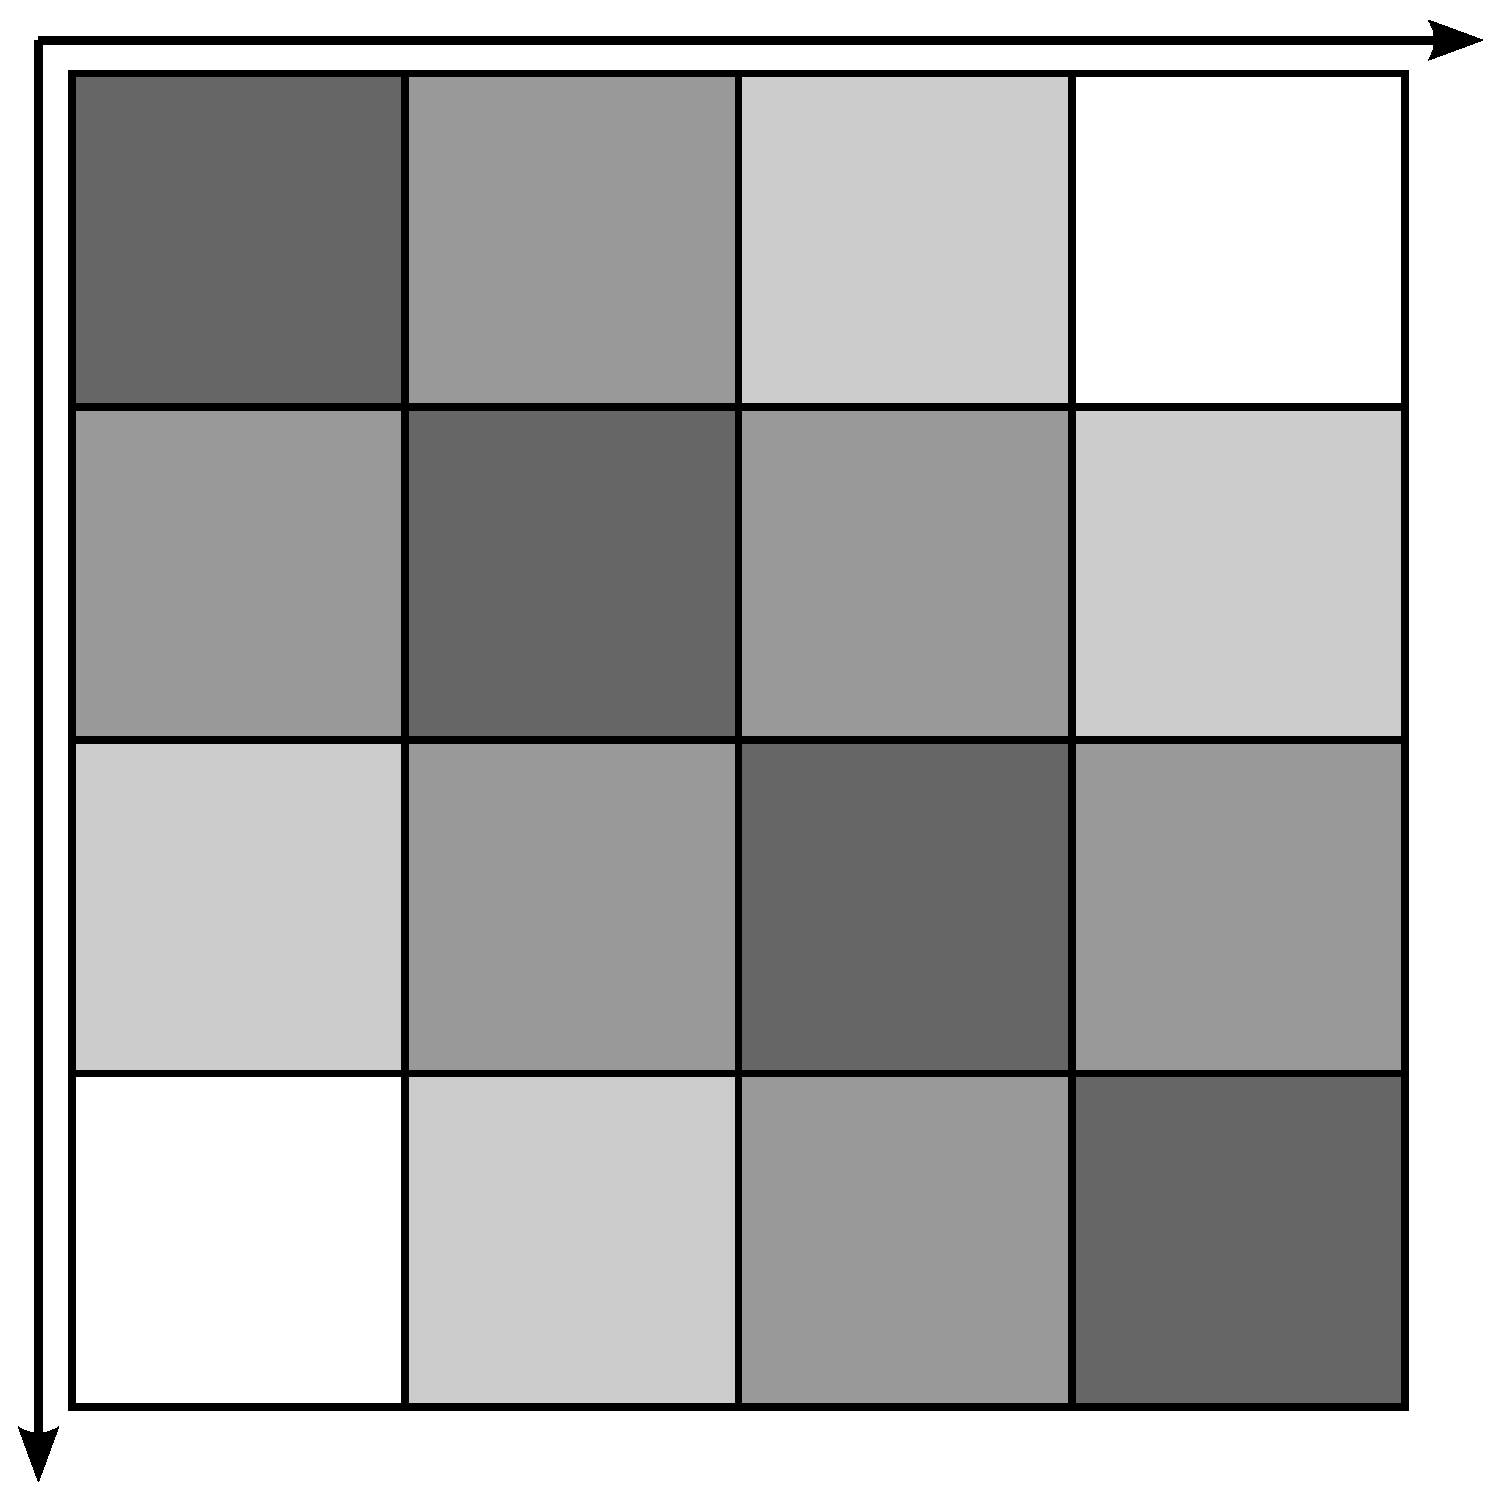
\includegraphics[width=0.46\unitlength]{proposal/doc/images/external/H_initial.eps}}
   \put(0.5400,0.0450){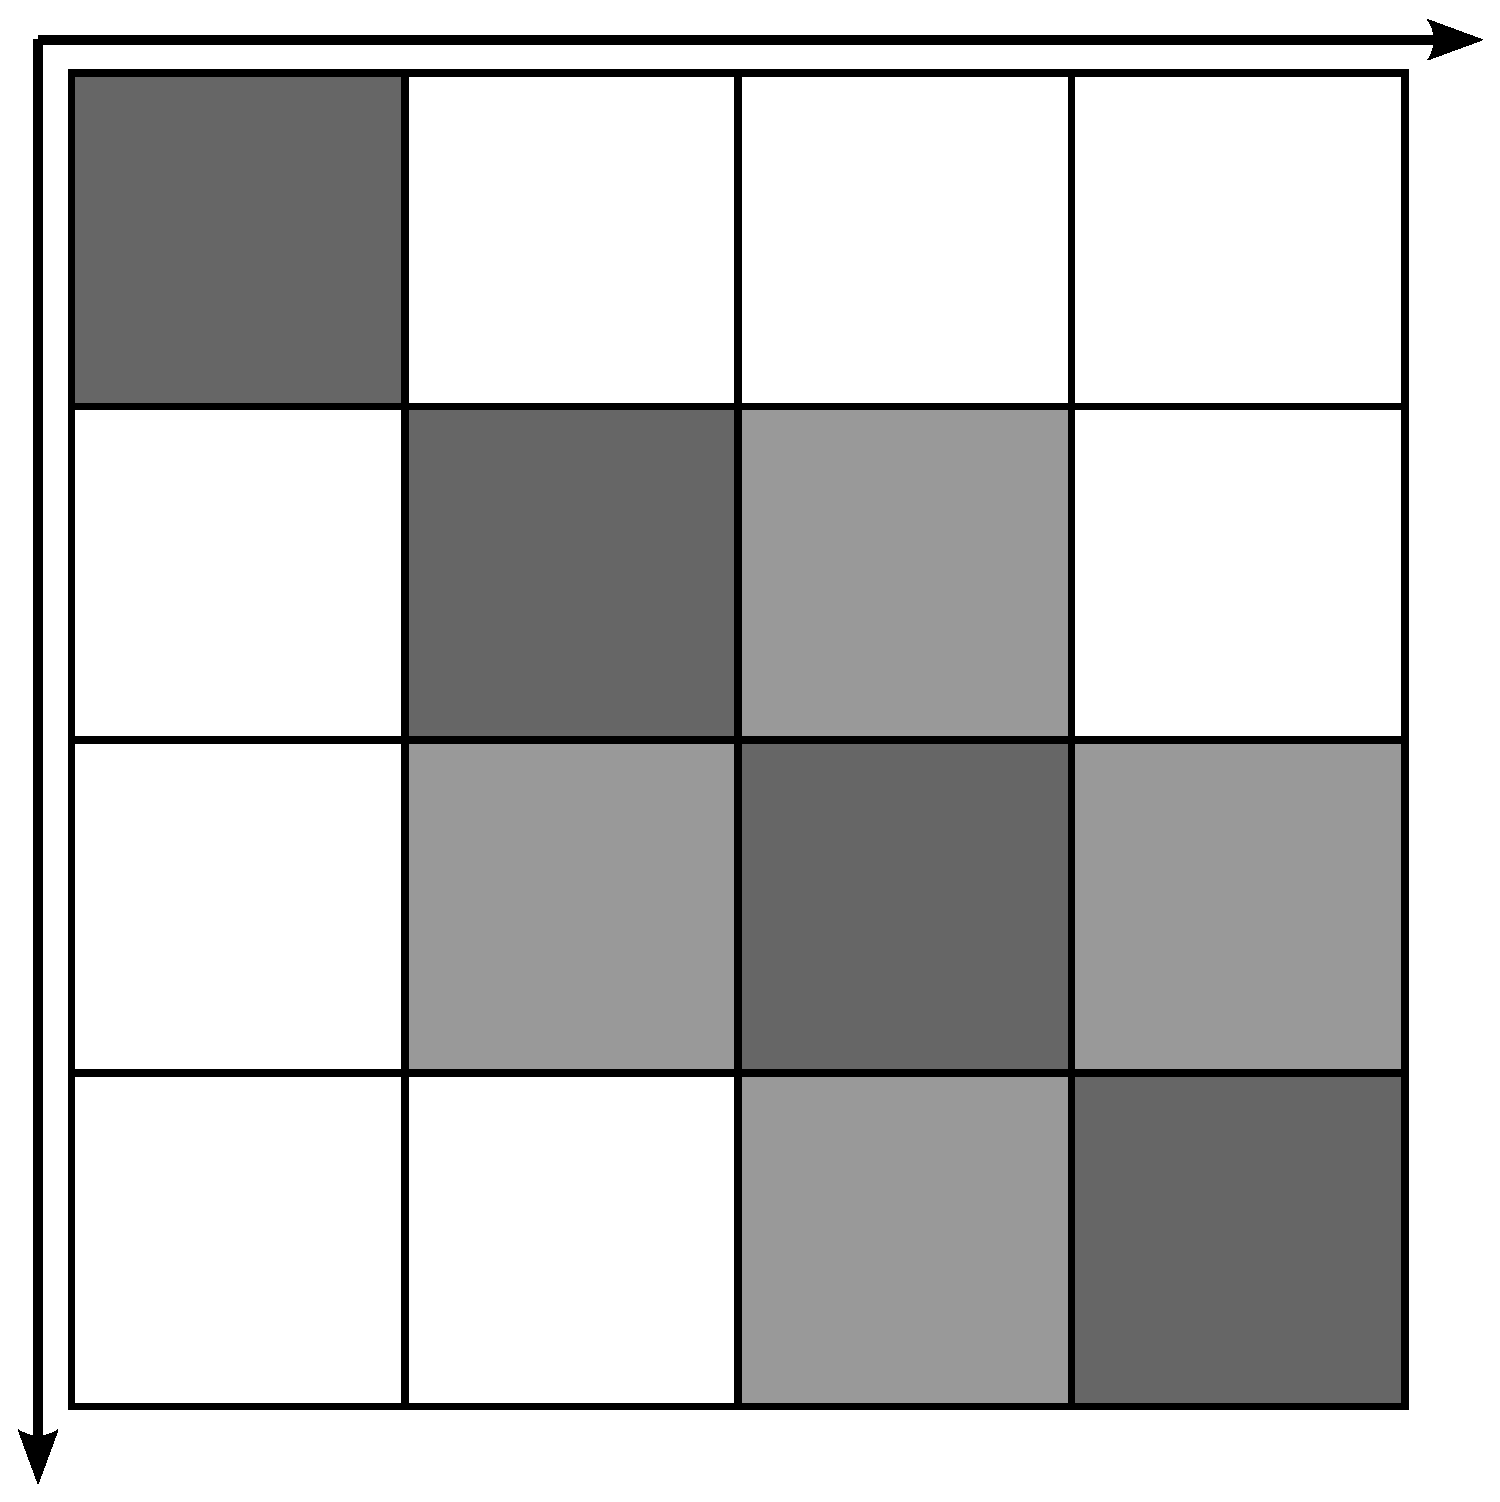
\includegraphics[width=0.46\unitlength]{proposal/doc/images/external/H_IMSRG_3ph_decoupling.eps}}
   \put(0.0100,0.0000){\parbox{0.5\unitlength}{\centering$\braket{i|H(0)|j}$}}
   \put(0.5200,0.0000){\parbox{0.5\unitlength}{\centering$\braket{i|H(\infty)|j}$}}

   \put(0.0500,0.5100){\parbox{0.11\unitlength}{\centering\footnotesize0p0h}}
   \put(0.1600,0.5100){\parbox{0.11\unitlength}{\centering\footnotesize1p1h}}
   \put(0.2630,0.5100){\parbox{0.11\unitlength}{\centering\footnotesize2p2h}}
   \put(0.3650,0.5100){\parbox{0.11\unitlength}{\centering\footnotesize3p3h}}
   \put(0.5500,0.5100){\parbox{0.11\unitlength}{\centering\footnotesize0p0h}}
   \put(0.6600,0.5100){\parbox{0.11\unitlength}{\centering\footnotesize1p1h}}
   \put(0.7630,0.5100){\parbox{0.11\unitlength}{\centering\footnotesize2p2h}}
   \put(0.8650,0.5100){\parbox{0.11\unitlength}{\centering\footnotesize3p3h}}
  %
   \put(0.0100,0.4320){\parbox{0.11\unitlength}{\rotatebox{90}{\centering\footnotesize0p0h}}}
   \put(0.0100,0.3235){\parbox{0.11\unitlength}{\rotatebox{90}{\centering\footnotesize1p1h}}}
   \put(0.0100,0.2175){\parbox{0.11\unitlength}{\rotatebox{90}{\centering\footnotesize2p2h}}}
   \put(0.0100,0.1100){\parbox{0.11\unitlength}{\rotatebox{90}{\centering\footnotesize3p3h}}}

   \put(0.5100,0.4320){\parbox{0.11\unitlength}{\rotatebox{90}{\centering\footnotesize0p0h}}}
   \put(0.5100,0.3235){\parbox{0.11\unitlength}{\rotatebox{90}{\centering\footnotesize1p1h}}}
   \put(0.5100,0.2175){\parbox{0.11\unitlength}{\rotatebox{90}{\centering\footnotesize2p2h}}}
   \put(0.5100,0.1100){\parbox{0.11\unitlength}{\rotatebox{90}{\centering\footnotesize3p3h}}}
  \end{picture}
    \\
    {\tiny Hergert, 2015}
  \end{center}

    \begin{itemize}
      \item{$\eta$ chosen so that $\refgnd{}$ is decoupled from $npnh$ excitations}
      % \item{Magnus expansion: solve for $U(s)=\exp(\Omega(s))$ directly}
      \item{MBPT corrections involve $\braket{\Phi | H | \Phi_{i\ldots}^{a\ldots}}$ and thus vanish}
    \end{itemize}
  \end{frame}

  \begin{frame}{$m$-scheme vs.\ $J$-scheme}
    For nuclear applications, choose HO-like single-particle basis:
    \begin{equation*}
      \ket{n_a (l_a s_a) j_a m_{j_a} t_a m_{t_a}} \equiv \ket{\alpha_a} \equiv \ket{\alpha_{\tilde{a}} m_{j_{\tilde{a}}}}
    \end{equation*}
    $m$-scheme - build antisymmetrized set of 2-body/3-body states:
    \begin{align*}
      \ket{\alpha_a \alpha_b} &\rightarrow \twobodyop{O}_{pqrs} \\
      \ket{\alpha_a \alpha_b \alpha_c} &\rightarrow \threebodyop{O}_{pqrstu}
    \end{align*}
    $J$-scheme - couple states to total $J$/$\mathcal{J}$:
    \begin{align*}
      \ket{(\alpha_{\tilde{a}} \alpha_{\tilde{b}})J M_{J}} &\rightarrow O_{\tilde{p}\tilde{q}\tilde{r}\tilde{s}}^{(2),J} \\
      \ket{[(\alpha_{\tilde{a}} \alpha_{\tilde{b}}) J \alpha_{\tilde{c}}] \mathcal{J} M_{\mathcal{J}}} &\rightarrow O_{\tilde{p}\tilde{q}\tilde{r}\tilde{s}\tilde{t}\tilde{u}}^{(3),J_1,J_2,\mathcal{J}}
    \end{align*}
    $J$-scheme matrix elements independent of $M_J$/$M_{\mathcal{J}}$
  \end{frame}

  % \section{Contributions}

  \begin{frame}{Outline of project}
    \begin{itemize}
      \item{Reimplement IM-SRG(2) and extend implementation to IM-SRG(3) in $m$-scheme}
      \item{Validate $m$-scheme implementation}
      \item{Implement IM-SRG(3) in $J$-scheme}
      \item{Validate $J$-scheme implementation against $m$-scheme implementation}
      \item{Study IM-SRG(3) contributions to ground-state properties of medium-mass nuclei}
    \end{itemize}
  \end{frame}

  \begin{frame}{IM-SRG(2):\ ${}^4\text{He}$}
    Start from intrinsic Hamiltonian with only NN force:
    \begin{equation*}
      H = T_{\text{int}} + \twobodyop{V}
    \end{equation*}
    Work with HO single-particle basis,\\
    and truncate at $e_{\text{max}} = 2 \ge 2 n + l$ \textcolor{gray}{(N = 40, large-scale N = 1820)}

    Benchmark: Ragnar Stroberg's IM-SRG(2) implementation

    What about IM-SRG(3)?
    \begin{itemize}
      \item{$\mathcal{O}(N^6)\,\text{storage resources} \sim 10\,\text{GB}$ \textcolor{gray}{($40^6 \times 8$ bytes)}}
      \item{$\mathcal{O}(N^9)\,\text{compute resources} \sim 100\,\text{TFLOPs}$ \textcolor{gray}{($40^9$ operations)}}
    \end{itemize}

    Comparsion: CCSD-T1 has $\mathcal{O}(N^7)$ computational cost
  \end{frame}

  \begin{frame}{IM-SRG(2):\ ${}^4\text{He}$ results}
    \begin{center}
      \centering
      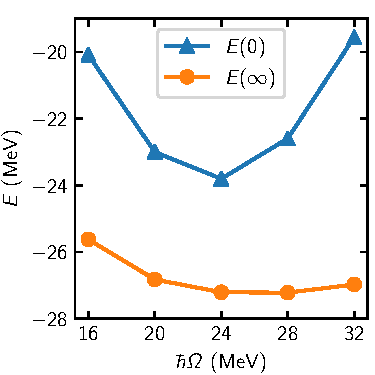
\includegraphics[width=0.45\textwidth]{proposal/talk/images/he4_imsrg2_energies.pdf}
      \hskip1em
      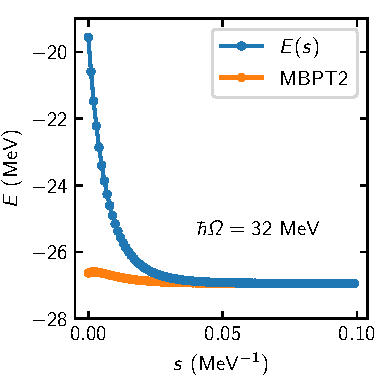
\includegraphics[width=0.45\textwidth]{proposal/talk/images/he4_imsrg2_flow.pdf}
    \end{center}
    \begin{itemize}
      \item{Second- and third-order MBPT corrections absorbed into E}
      \item{Agreement with Stroberg up to $10^{-5}\,\text{MeV}$}
    \end{itemize}
  \end{frame}

  \begin{frame}{IM-SRG(3):\ pairing Hamiltonian}
    Hamiltonian with 2-fold degenerate levels \\
    with (attractive) pairing interaction:
    \begin{equation*}
      H = \delta \sum_{p \sigma} (p - 1)\crea{p\sigma} \annih{p\sigma}
      - \frac{g}{2} \sum_{pq} \crea{p+}\crea{p-}\annih{q-}\annih{q+}
    \end{equation*}
    Fix $\delta=1\mev$, consider 4 particles in 4 levels

    Choose reference state with 2 lowest levels filled:
    \begin{itemize}
      \item{Reference state is the Hartree-Fock Slater determinant}
      \item{Has Hartree-Fock energy $E_{\text{HF}} = 2 - g$ (for $A=4$)
        % \textcolor{gray}{($\delta (\frac{A}{2} - 1) \frac{A}{2} - \frac{g}{4}{\left(\frac{A}{2}\right)}^2$ in general)}
        }
      \item{IM-SRG needs to bring in correlation effects}
    \end{itemize}
    \begin{equation*}
      E_{\text{corr}} = E_{\text{exact}} - E_{\text{HF}} = E(\infty) - E(0)
    \end{equation*}
  \end{frame}

  \begin{frame}{IM-SRG(3):\ pairing Hamiltonian results}
    \begin{center}
      \centering
      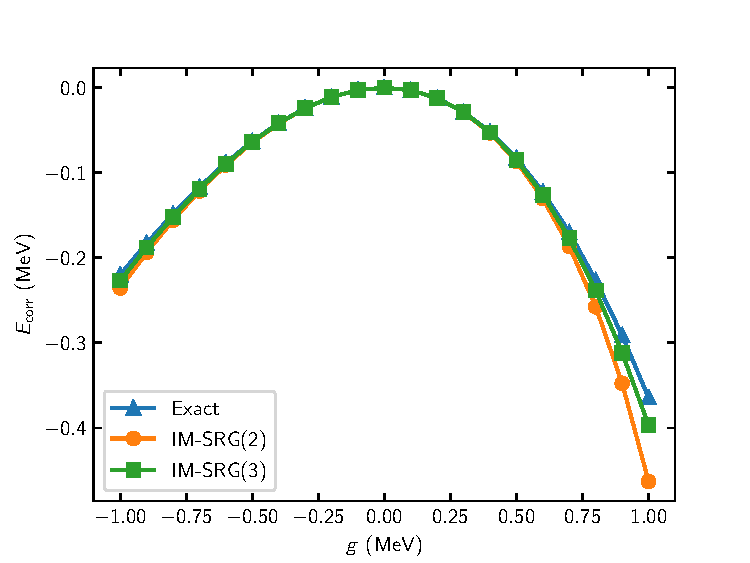
\includegraphics[width=0.8\textwidth]{proposal/talk/images/pairing_ham_imsrg3.pdf}
    \end{center}
    \vskip-1em
    \begin{itemize}
      \item{See systematic improvement in correlation energy}
      \item{IM-SRG(3) helps with expansion convergence for large $g$}
    \end{itemize}
  \end{frame}

  \begin{frame}{Outlook}
    Accomplished so far:
    \begin{itemize}
      \item{Implemented general ($m$-scheme) IM-SRG(2)/(3)}
      \item{Validated implementation against previous calculation \\
        and exactly solvable pairing Hamiltonian}
    \end{itemize}
    Next steps:
    \begin{itemize}
      \item{Implement $J$-scheme IM-SRG(3) commutators}
      \item{Validate implementation against $m$-scheme commutators}
      \item{Optimize performance to extend basis truncation}
      \item{Study medium-mass closed-shell nuclei (${}^{40}\text{Ca}$)}
    \end{itemize}

    \pause
    \begin{center}
    \textbf{Thank you for your attention}
    \end{center}
  \end{frame}

\end{document}
